% Filename: Methods.tex
% Last update: Monday, 11/5/2018 by Ally Warner
%%%%%%%%%%%%%%%%%%%%%%%%%%%%%%%%%%%%%%%%%%%%%%%%%%%%%%%%%%%%%%%%%%%%%%

\section{Methods}
\label{sec:Methods}

In this section, we describe in detail all of the steps of the modeling pipeline (Figure \ref{fig:pipeline}). We begin with data acquisition of $T_1$ and $T_2$ MRIs, DWI, fMRI, and EEG followed by image pre-processing. After the images have been pre-processed, the MRIs are segmented into eight tissue layers to create a three-dimensional tetrahedral mesh. All of the image modalities are registered to a common coordinate space and used for forward problem simulations with the processed EEG data.

%%Pipeline figure
\begin{figure}[H]
    \centering
    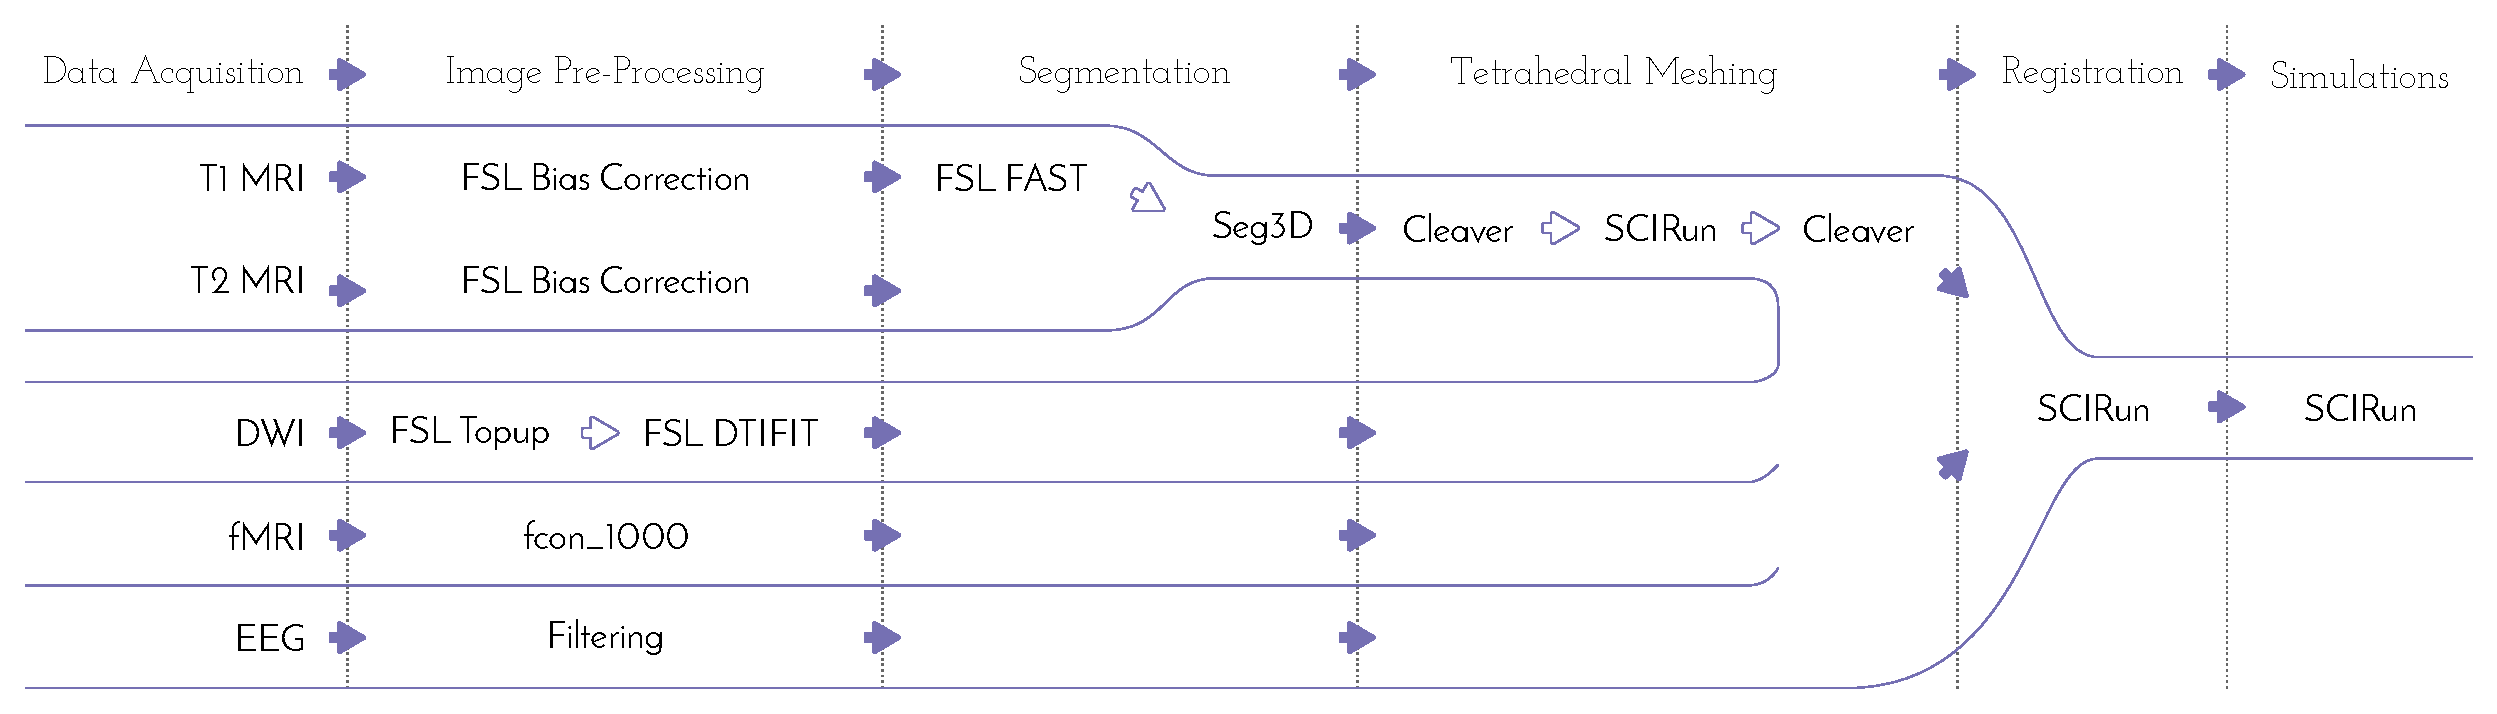
\includegraphics[width=\textwidth]{Figures/pipeline}
    \caption{Comprehensive head/brain model pipeline. Data sources are shown on the left with software packages used for creating the head/brain model in the middle and the simulation software on the right.}
    \label{fig:pipeline}
\end{figure}

\subsection{Data Acquisition}
\label{sec:Data}

%%% Image and EEG Acquisitions 

To construct a high-resolution, personalized, anisotropic volume conductor whole-head model, $T_1$-, $T_2$- weighted, diffusion weighted, and functional magnetic resonance images (MRI) were acquired on a healthy female subject, 23 years of age, on a Skyra 3T full-body scanner (Siemens Medical Solutions, Erlangen, Germany).

The $T_1$-weighted scan was performed with a three-dimensional magnetization-prepared, rapid gradient echo (MPRAGE) sequence \cite{ref:mprage}. The parameters used were as follows: echo time: 3.41ms; repetition time: 2500ms; flip angle: 7 $^{\circ}$; resolution matrix size: 256x256 pixels; field of view: 256mm; 208 sagittal slices with a slice thickness of 1mm. Acquisition time was 10:42 minutes.

The $T_2$-weighted scan was performed with a SPACE (sampling perfection with application)-optimized contrast using different flip angle evolutions - sequence \cite{ref:space}. The parameters used were as follows: echo time: 406ms; repetition time: 3200ms; resolution matrix size: 256x256 pixels; field of view: 256mm; 208 sagittal slices with a slice thickness of 1mm. Acquisition time was 5:34 minutes. The subject did not move in between the two scans so the scans did not need to be registered.

The diffusion weighted images (DWI) were acquired with multiband, two-dimensional, echo-planar imaging (EPI) \cite{ref:epi}. Both phase-encoding directions were performed (anterior to posterior and posterior to anterior) with 64 diffusion directions each. Further sequence parameters for each scan were as follows: echo time: 76.8ms; repetition time: 4070ms; flip angle: 90 $^{\circ}$; resolution matrix size: 104x104 pixels; field of view: 208mm; 60 slices with 2.5mm slice thickness. Acquisition time was 5:05 minutes each.

The functional MRI (fMRI) scans were acquired with a blood oxygenation level dependent contrast (BOLD) sequence. The following parameters were used: echo time: 76.8ms; repetition time: 780ms; flip angle: 55 $^{\circ}$; resolution matrix size: 104x104 pixels; field of view: 210mm; 72 slices with 2mm slice thickness. Acquisition time was 10:32 minutes.

Continuous electroencephalograms (EEGs) were recorded using a 128-channel and 256 channel HydroCel Geodesic Sensor Net that was connected to a NetAmps 400 amplifier and referenced online to a single vertex electrode. Channel impedances were kept at or below 50 kOhms and signals were sampled at 250Hz. The EEGs were recorded while the subject sat quietly in a chair, alternating two-minute epochs of eyes open and eyes closed, for a total of twelve minutes.

All acquisition reports will be included with the dataset.

\subsection{Preprocessing of Images}
\label{sec:preprocess}

%FSL
\begin{wrapfigure}[16]{hr}{3cm}
    \centering
    \vspace{-63pt}
    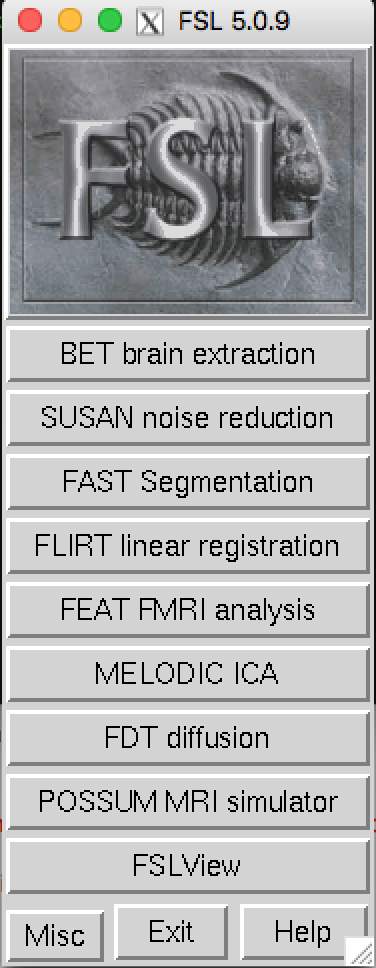
\includegraphics[width=3cm]{Figures/FSL}
    \caption{FMRIB software library user interface.}
    \label{fig:fsl}
\end{wrapfigure}

\subsubsection{MRI Correction}

Bias field signal is a low-frequency, smooth signal that corrupts MRI images due to inhomogeneities in the magnetic fields of the MRI machine by blurring images, thereby reducing the high frequencies of the images, such as edges and contours. The signal changes the intensity values of image pixels so that the same tissue has a different distribution of grayscale intensities across the image. \cite{ref:bias} We applied an estimated bias field correction on the $T_1$ and $T_2$ MRIs using FMRIB Software Library (FSL) FAST \cite{ref:fslfast}, which will be further described in Section \ref{sec:Seg}.

\subsubsection{DWI Distortion Correction}

DWIs performed with EPI sequences are prone to distortions from rapid switching of diffusion weighting gradients, movement from the scanning table, and movement from the subject. The diffusion data was collected with reversed phase-encoded blips (anterior to posterior (AP) and posterior to anterior (PA)), resulting in pairs of images with distortions in opposite directions. From these pairs, we estimated the susceptibility-induced off-resonance field using a method \cite{ref:fsltopup1} similar to what is currently implemented in FSL.\cite{ref:fsltopup2} We then combined the two images into a single corrected one using FSL's topup and eddy command line tools. Details on this process are described in the Appendix in Section \ref{sec:distortion}.

\subsubsection{Diffusion Tensor Images}

After we corrected the DWI images, we calculated diffusion tensor images (DTI) using FSL's DTIFIT toolbox \cite{ref:dtifit}. We then used SCIRun \cite{ref:scirun} to build the conductivity tensor field,as described in section 2.5.1, from the eigenvectors and eigenvalues output from DTIFIT. Details on using DTIFIT are described in the Appendix in Section \ref{sec:dtifit}.

\begin{figure}[H]
\begin{center}
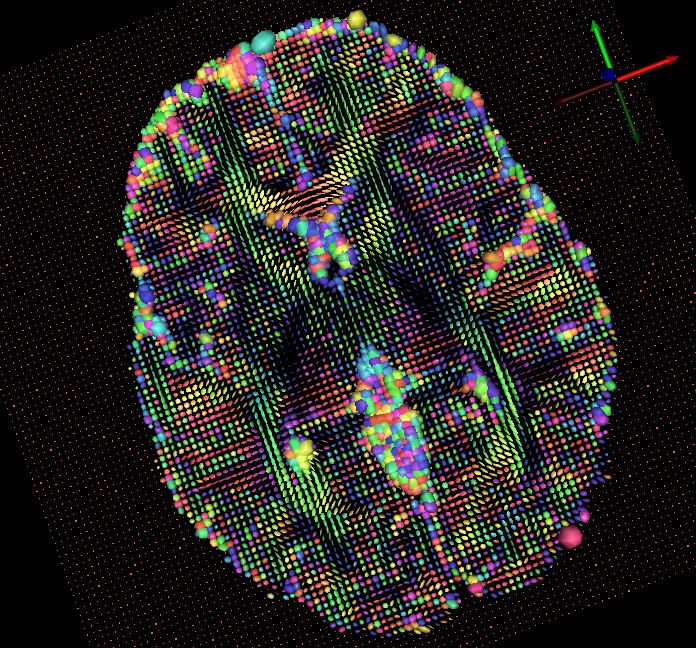
\includegraphics[width=0.75\textwidth]{Figures/DTI_1.png}
\caption{Diffusion tensor visualization using SCIRun.}
\label{fig:tensorvis}
\end{center}
\end{figure}

\begin{figure}[H]
\begin{center}
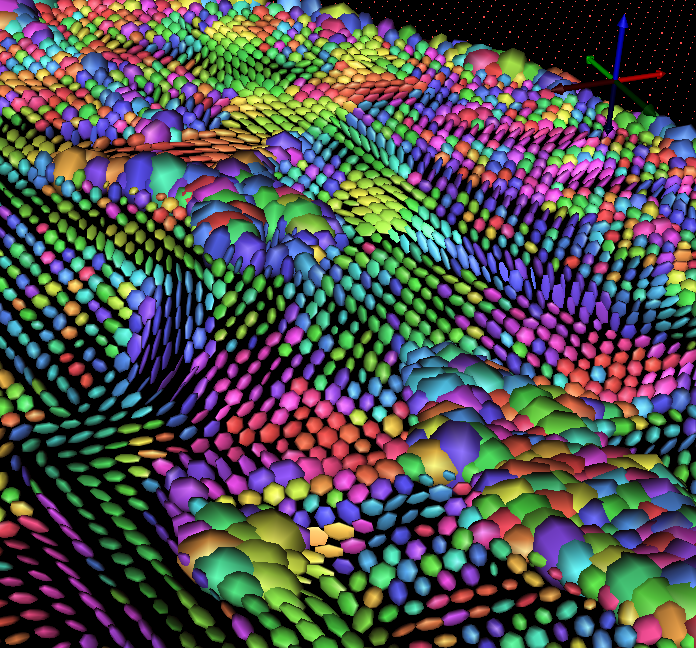
\includegraphics[width=0.75\textwidth]{Figures/DTI_2.png}
\caption{Diffusion tensor visualization using SCIRun.}
\label{fig:tensorvis2}
\end{center}
\end{figure}

We built the tensor field in SCIRun rather than in 3D Slicer \cite{ref:slicer} or FSL DTIFIT because the output data had a different orientation and could not be easily registered with the mesh in SCIRun.

\begin{figure}[H]
\begin{center}
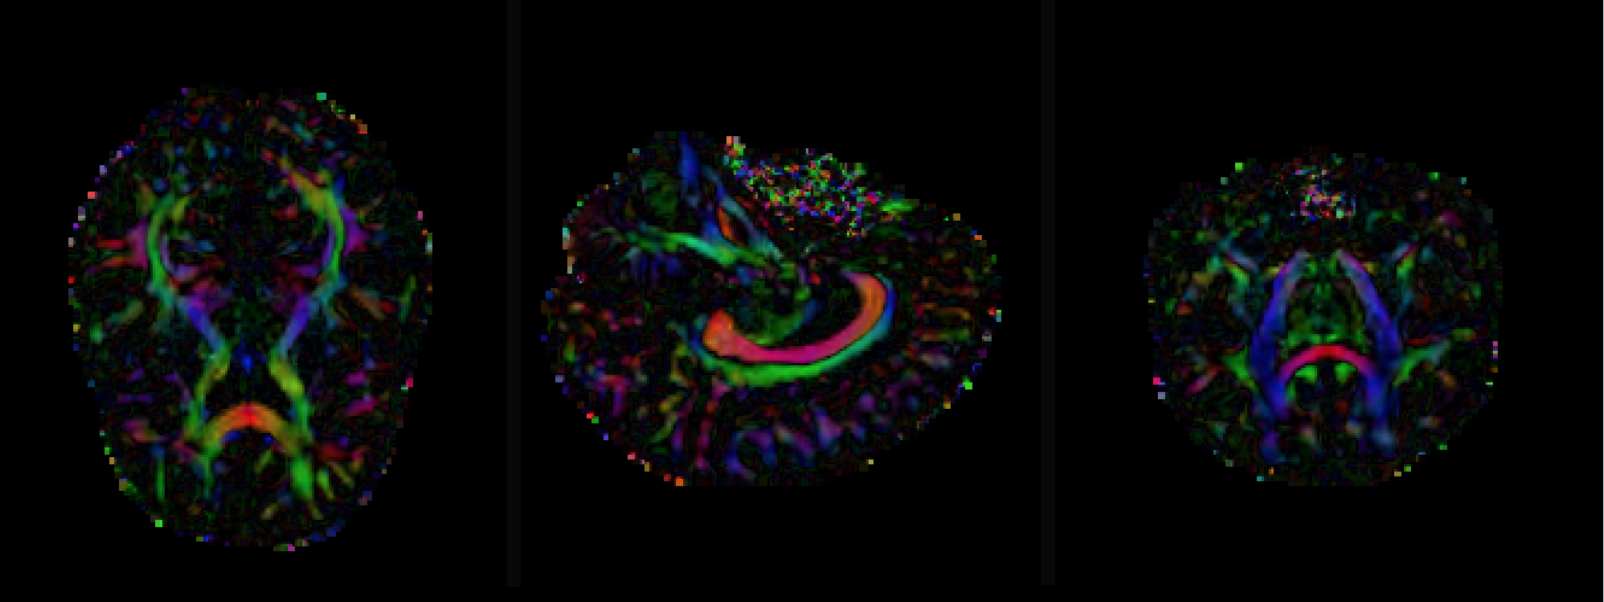
\includegraphics[width=0.75\textwidth]{Figures/backwards.png}
\caption{Example of difference in orientation between SCIRun and 3D
  Slicer data.}
\label{fig:backwards}
\end{center}
\end{figure}

\subsubsection{fMRI}
\label{sec:fmripre}

We preprocessed the fMRI data using the 1000 Functional Connectomes (fcon) Project pipeline scripts \cite{ref:fcon}, which performed anatomical preprocessing, functional preprocessing, registration to the $T_1$ MRI, segmentation, and nuisance signal regress. The outline pipeline used on this fMRI dataset, specific to the University of Utah, can be found at \url{https://bitbucket.org/UtahBrainNetworks base_prep}, which includes instructions for installation, compilation, and usage. The preprocessed fMRI data was then converted from a four-dimensional dataset to a two-dimensional dataset to be visualized in SCIRun. The data conversion is described in the Appendix in Section \ref{sec:nifti}. 

\subsubsection{EEG}

A 60Hz notch filter and its harmonics \cite{ref:filter} were applied to the EEG data, and we created an EEG data matrix. The rows of the matrix corresponded to the channels of the EEG and the columns corresponded to the time step. We removed the last two rows of the EEG signals matrix as these were control rows for the experiment. We also removed several columns at the beginning and the end of the matrix, because these columns corresponded to taking the EEG net on and off the subject's head. The EEG data matrix is described in the Appendix in Section \ref{ref:eegmatlab}. 

\subsubsection{Registration}
\label{sec:reg}

Since the subject did not move in between the $T_1$ and $T_2$ MRI, no registration was necessary before segmentation and meshing. We generated the tetrahedral mesh from the segmentation and registered the mesh to the DTI coordinate space with a manual, rigid registration using SCIRun. We registered the fMRI data to the mesh coordinate space with a manual, rigid registration, using SCIRun as well. We included the registration transformation matrix to the DTI coordinate space in the dataset. The SCIRun networks for registration are included in the Appendix in Section \ref{sec:networks}

\begin{figure}[H]
\begin{center}
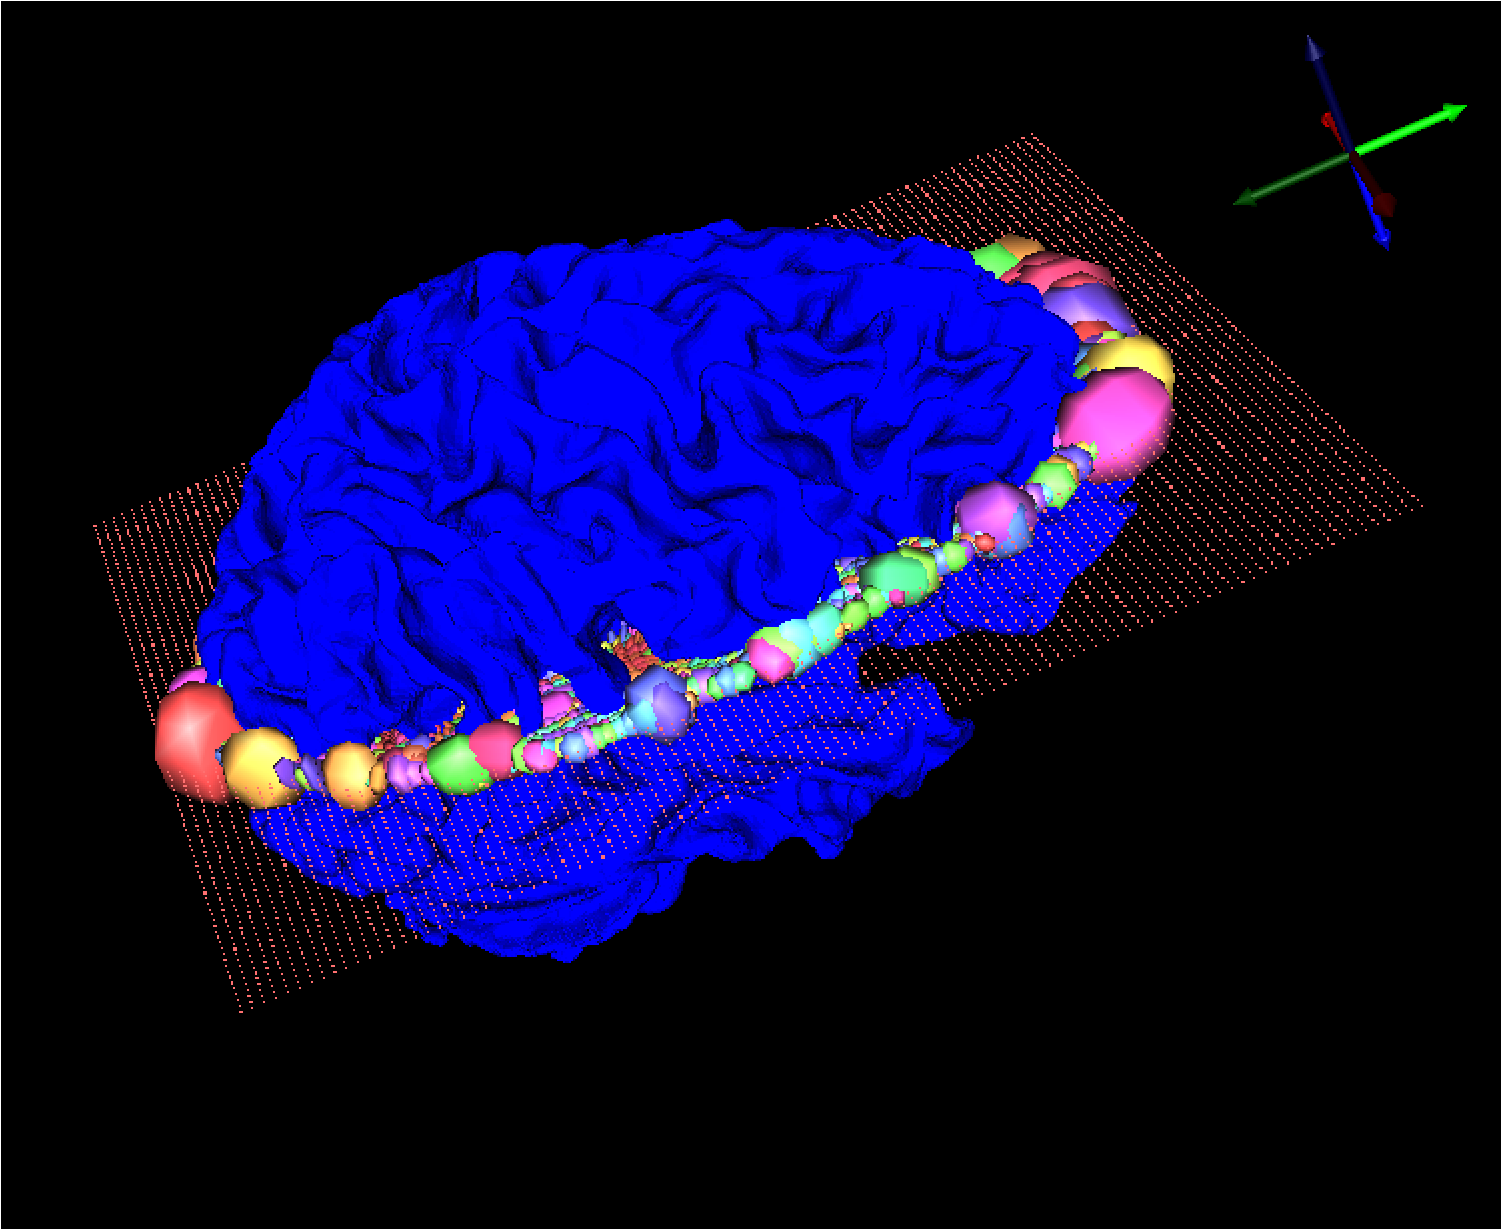
\includegraphics[height = 2.5in]{Figures/DTI_reg}
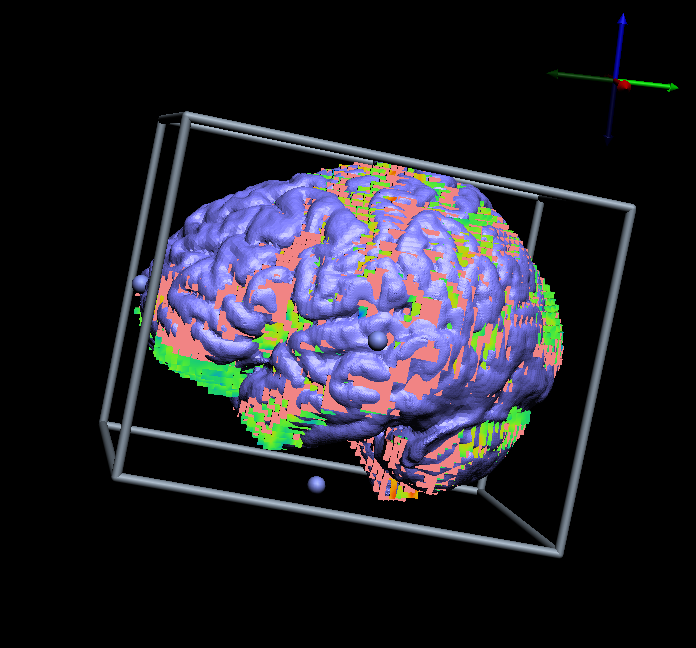
\includegraphics[height = 2.5in]{Figures/fmri_reg}
\caption{SCIRun manual registrations: mesh to DTI registration \textit{(left)}, fMRI to mesh registration \textit{(right)}.}
\label{fig:dtireg}
\end{center}
\end{figure}

\subsection{MRI Segmentation of Tissues}
\label{sec:Seg}

%%% Preparation for segmentation, trials, manual work 

Segmentation of the head tissues proved to be the most time-consuming portion of the pipeline. We segmented the head volume using FSL and Seg3D, a free volume segmentation and processing tool, \cite{ref:seg3d} into air, cerebral spinal fluid (CSF), white matter, gray matter, skull, sinus, eyes, and scalp. Segmentation of the brain was difficult due to the similar grayscale intensities across different tissues; thresholding the image produced noisy and incomplete layers. Segmentation of the sinuses and skull was also difficult because they are represented by only black pixels, with no clear tissue boundaries.

We generated the initial segmentation with FSL from the $T_1$ MRI by stripping the skull with the brain extraction tool (BET) \cite{ref:bet1}, and then with FAST segmentation. FSL FAST outputs grayscale probability images of CSF, white matter, and gray matter layers as well as a bias-corrected $T_1$ MRI. This method, compared with Freesurfer \cite{ref:freesurf}, Statistical Parametric Mapping through Matlab (SPM) \cite{ref:spm}, Atlas Based Classification through 3D Slicer \cite{ref:abc}, and Seg3D methods alone, produced the most qualitatively accurate initial brain segmentation results for this data.

\begin{figure}[H]
    \centering
    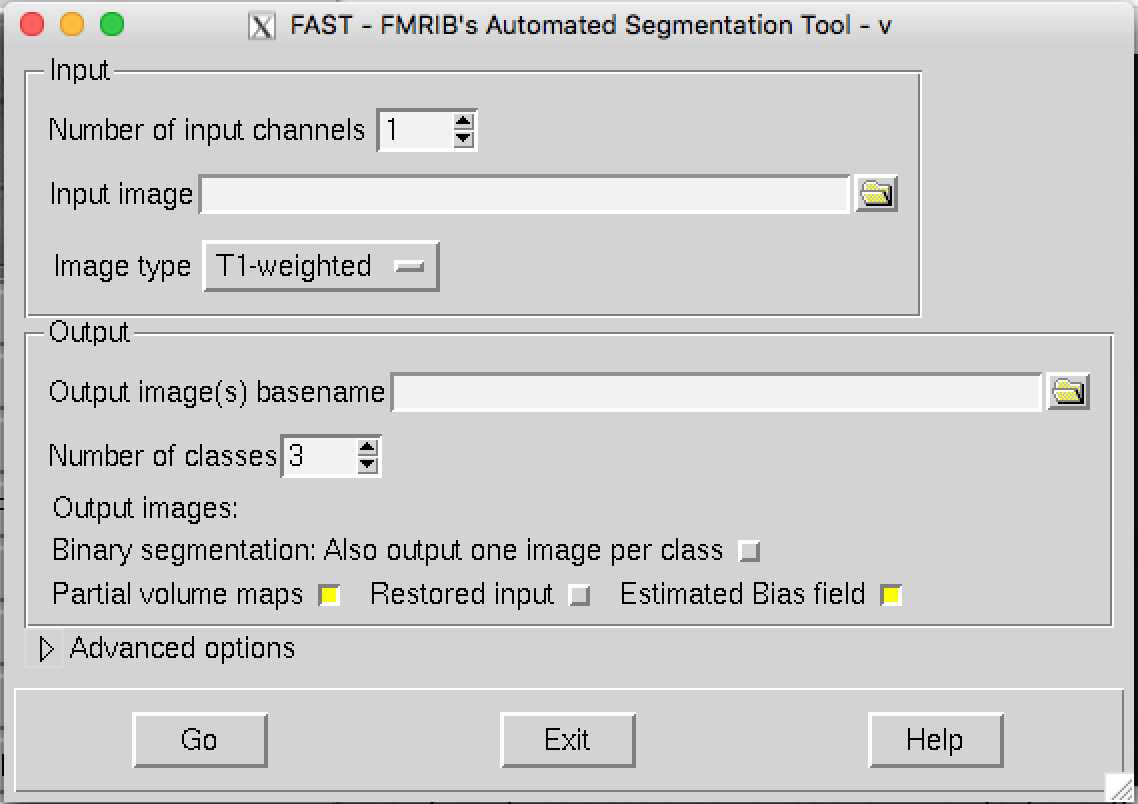
\includegraphics[width=.8\textwidth]{Figures/FSL_FAST}
    \caption{FSL FAST user interface.}
    \label{fig:fslfast}
\end{figure}

\begin{figure}[H]
\begin{center}
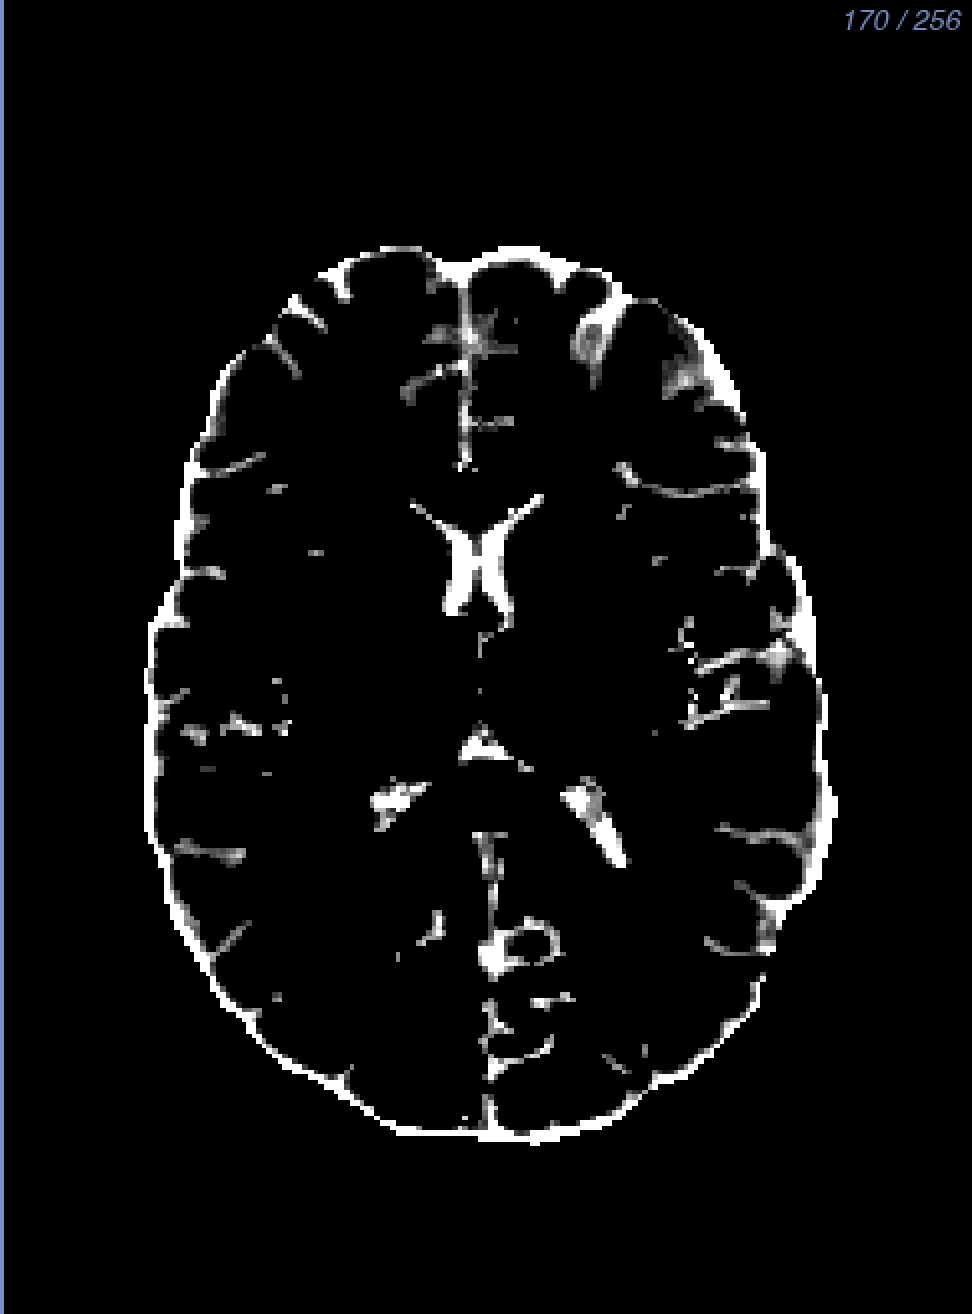
\includegraphics[width=.32\textwidth]{Figures/FSLFAST_csf}
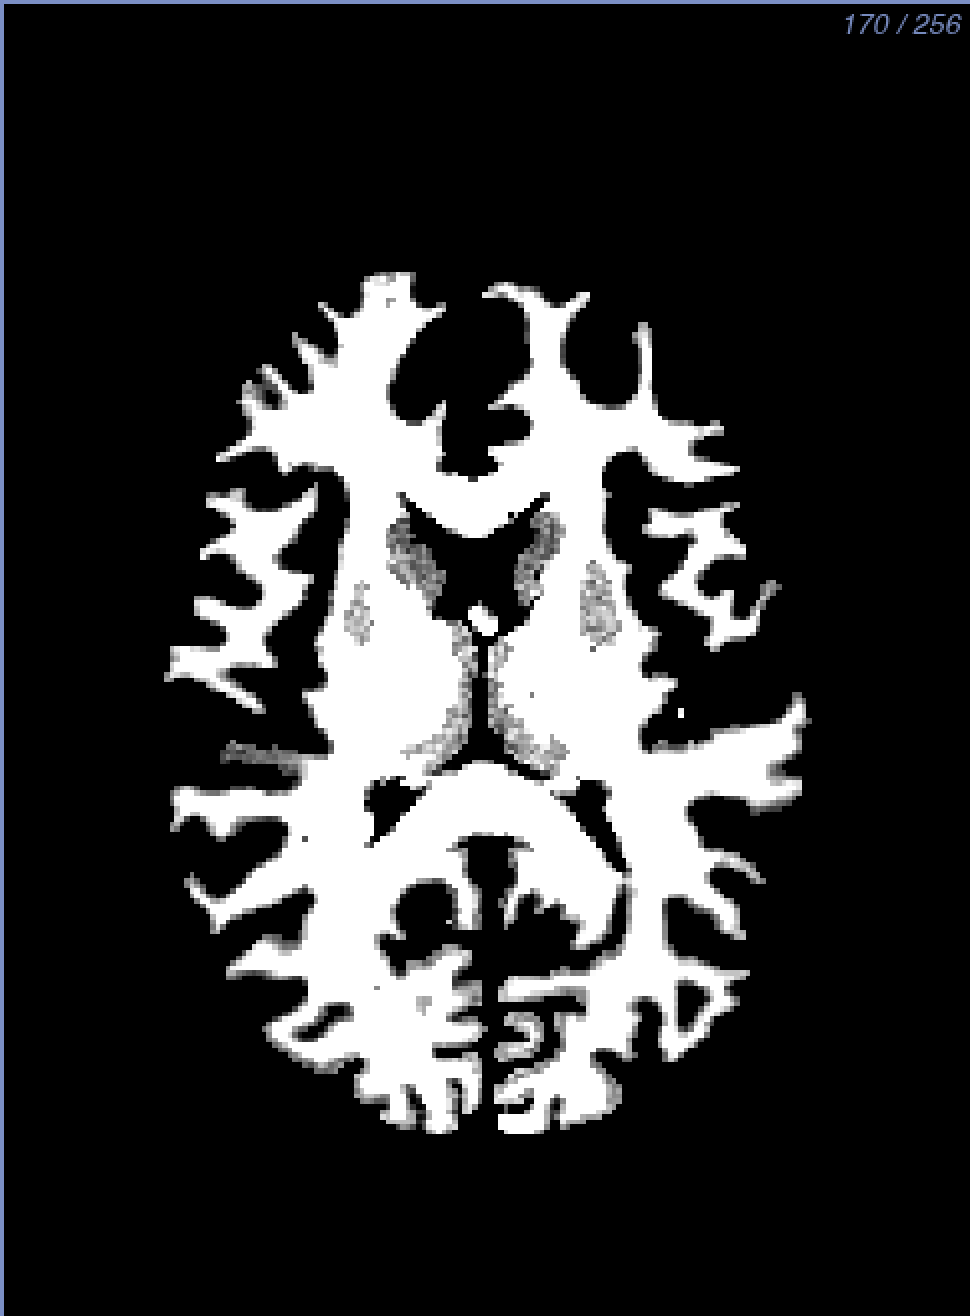
\includegraphics[width=.32\textwidth]{Figures/FSLFAST_wm}
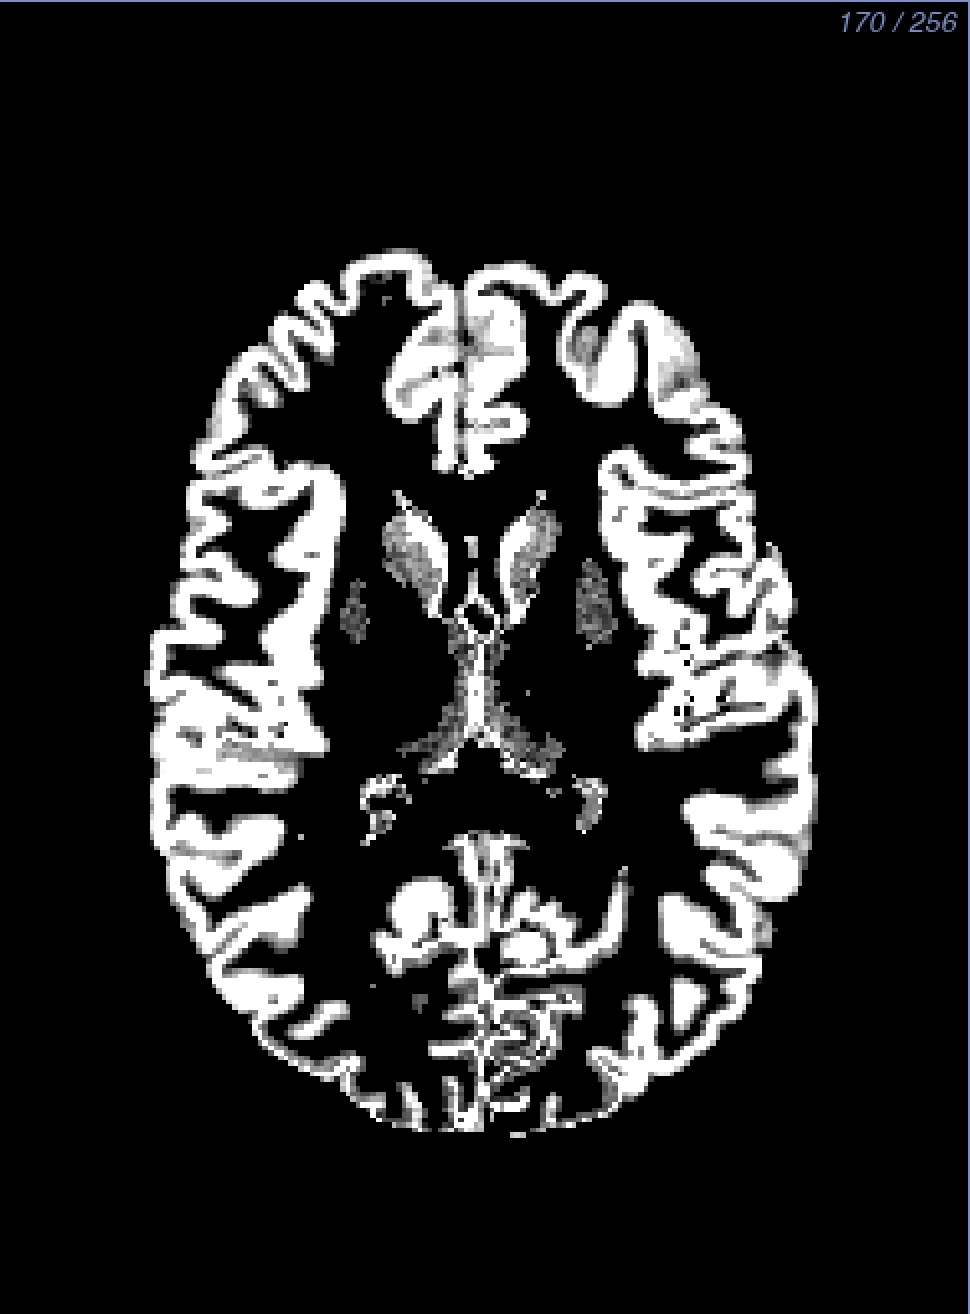
\includegraphics[width=.32\textwidth]{Figures/FSLFAST_gm}
\caption{FSL FAST output: CSF \textit{(left)}, white matter \textit{(center)}, gray matter \textit{(right)}.}
\label{fig:fastout}
\end{center}
\end{figure}

Although the FSL FAST results were an improvement compared to the other segmentation software trials, we manually improved the layers to add more detail and to remove any crossover between the layers. We started with the white matter layer because it is the innermost layer. First, we created a threshold layer FSL FAST output. We then inspected and manually edited each slice in every direction to add more detail or to clean up noise from FSL FAST.

\begin{figure}[H]
\begin{center}
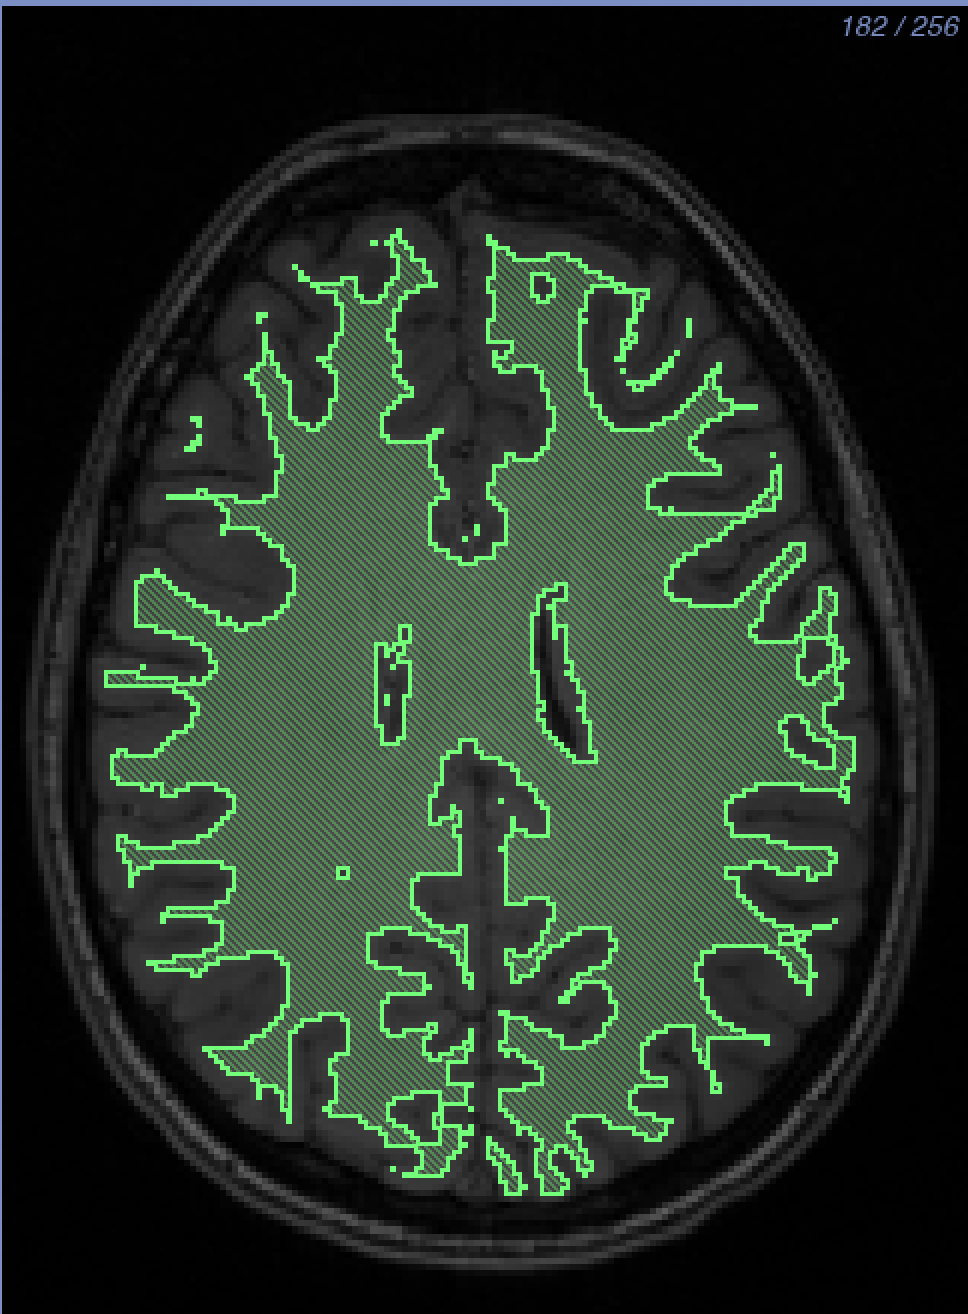
\includegraphics[width=.49\textwidth]{Figures/whitematter_before}
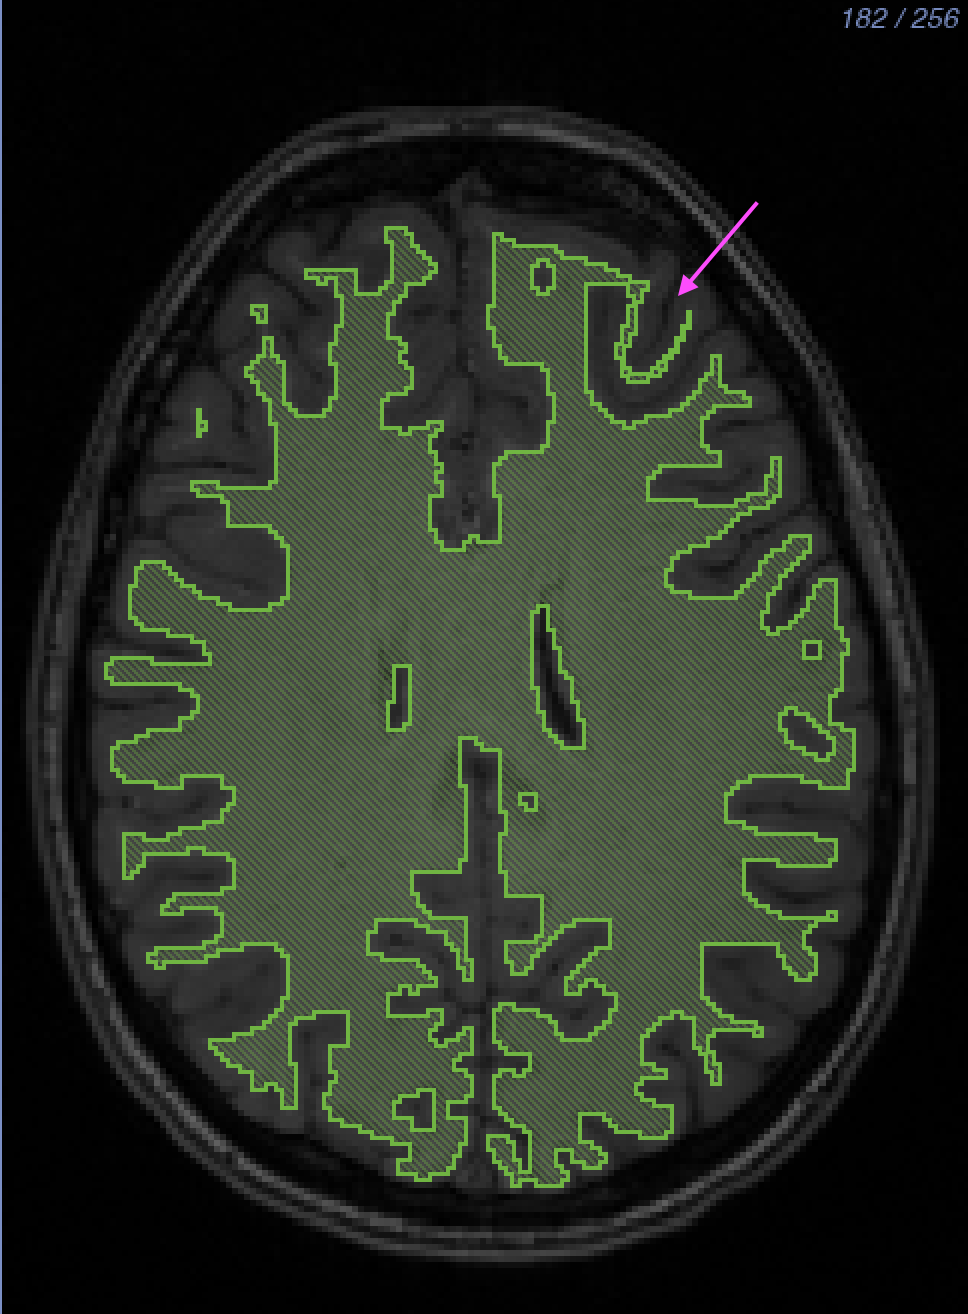
\includegraphics[width=.49\textwidth]{Figures/whitematter_after}
\caption{White matter segmentation: Before \textit{(left)} and after \textit{(right)} manual segmentation. The hook feature in the upper right-hand corner is a notable change between the two layers. The layer is more full and has less noise.}
\label{fig:wm}
\end{center}
\end{figure}

After we segmented the white matter, we created a threshold layer from the FSL FAST output for the gray matter. We inspected and manually edited each slice in every direction of the gray matter. We then removed the white matter layer from the gray matter using a Boolean remove mask filter to ensure no overlap between the layers. We manually filled any holes between the two layers. Lastly, we added a gray matter nuclei to the gray matter layer. The thresholding algorithms in Seg3D produced noise around these nuclei because of the similarities of the grayscale values. To fix this noise, we segmented the entire nuclei manually using the paintbrush tool in Seg3D. Then, we added the nuclei to the gray matter layer using a Boolean OR mask filter, and removed any overlap from the white matter layer using a Boolean remove mask filter.

\begin{figure}[H]
\begin{center}
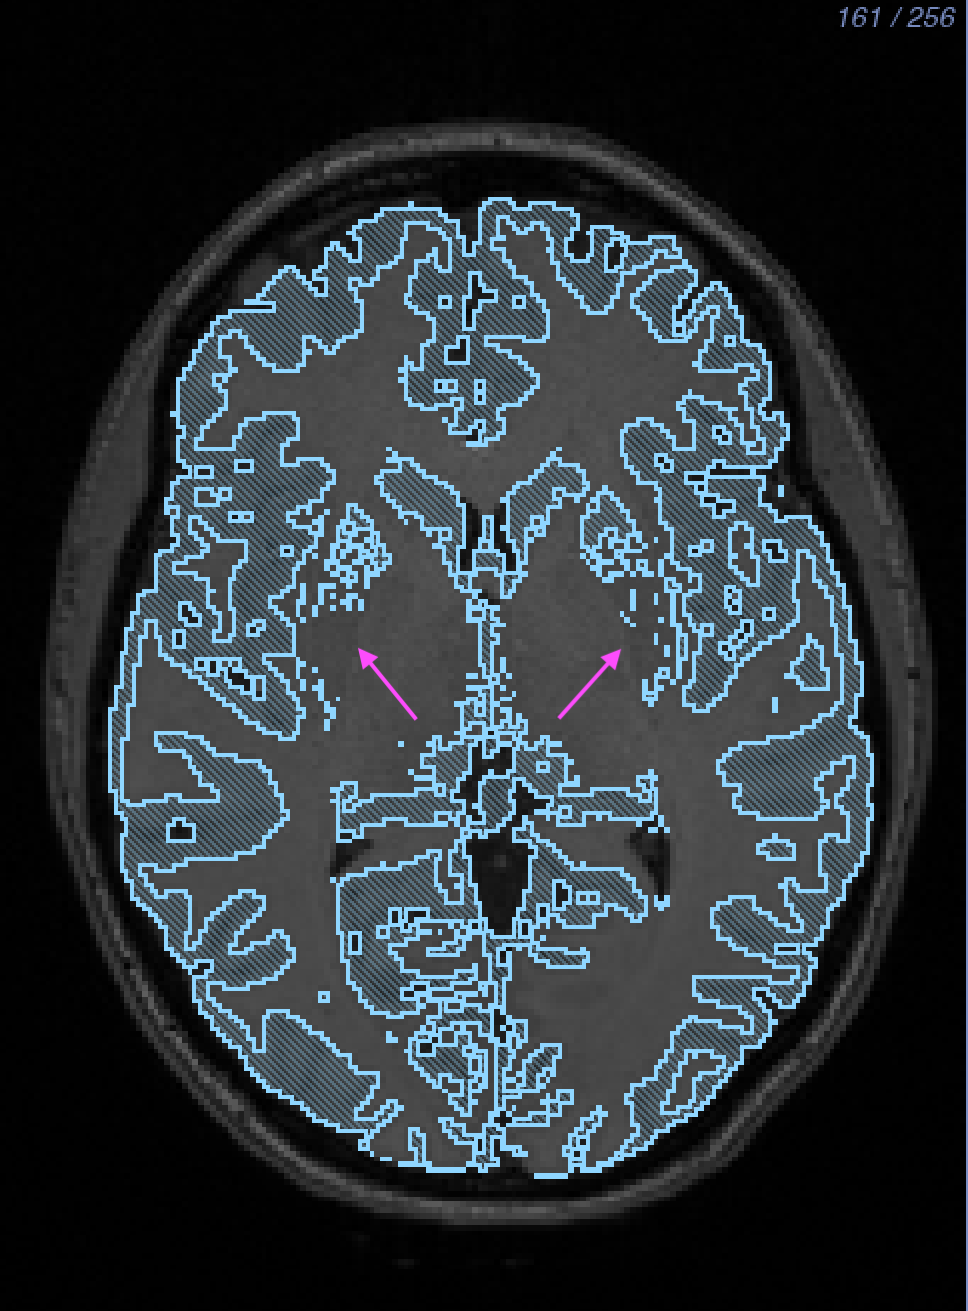
\includegraphics[width=.49\textwidth]{Figures/greymatter_before_nuclei}
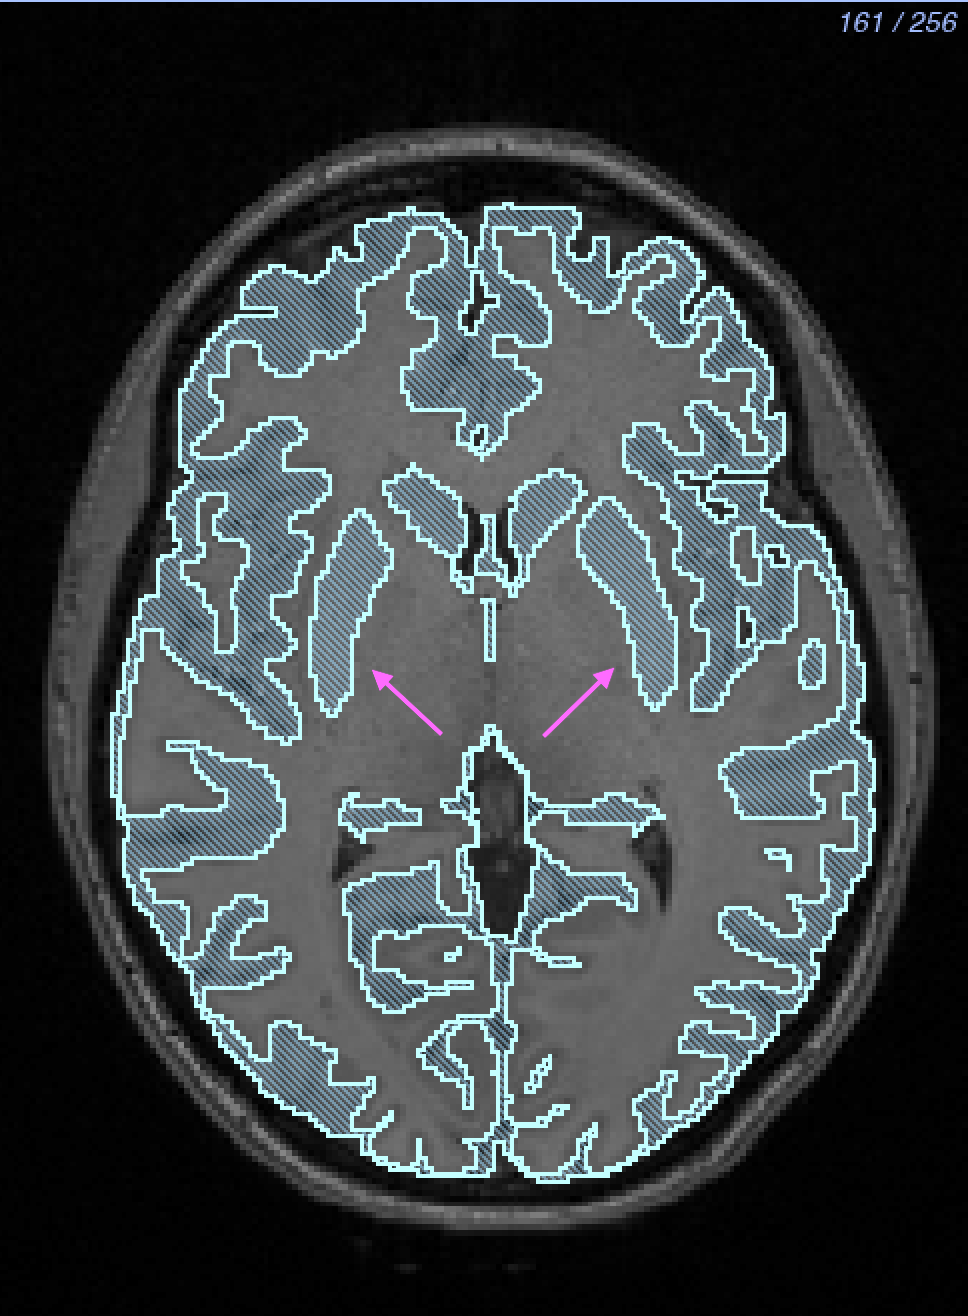
\includegraphics[width=.49\textwidth]{Figures/greymatter_added_nuclei}
\caption{Gray matter segmentation: Before \textit{(left)} and after \textit{(right)} manual segmentation. Gray matter nuclei located in the center of the brain were segmented manually.}
\label{fig:gm}
\end{center}
\end{figure}

After we completed the segmentation of the gray and white matter layers, we made the CSF layer by creating a solid threshold layer for the entire brain and removing the white and gray matter layers using a Boolean remove mask filter. We then checked the white matter, gray matter, and CSF layers for holes, both on the surface and inside the segmentation between layers. We also performed a manual, quality check on the layers to ensure that they were at least two pixels wide throughout. This thickness criteria helped create a tetrahedral mesh without holes.

\begin{figure}[H]
\begin{center}
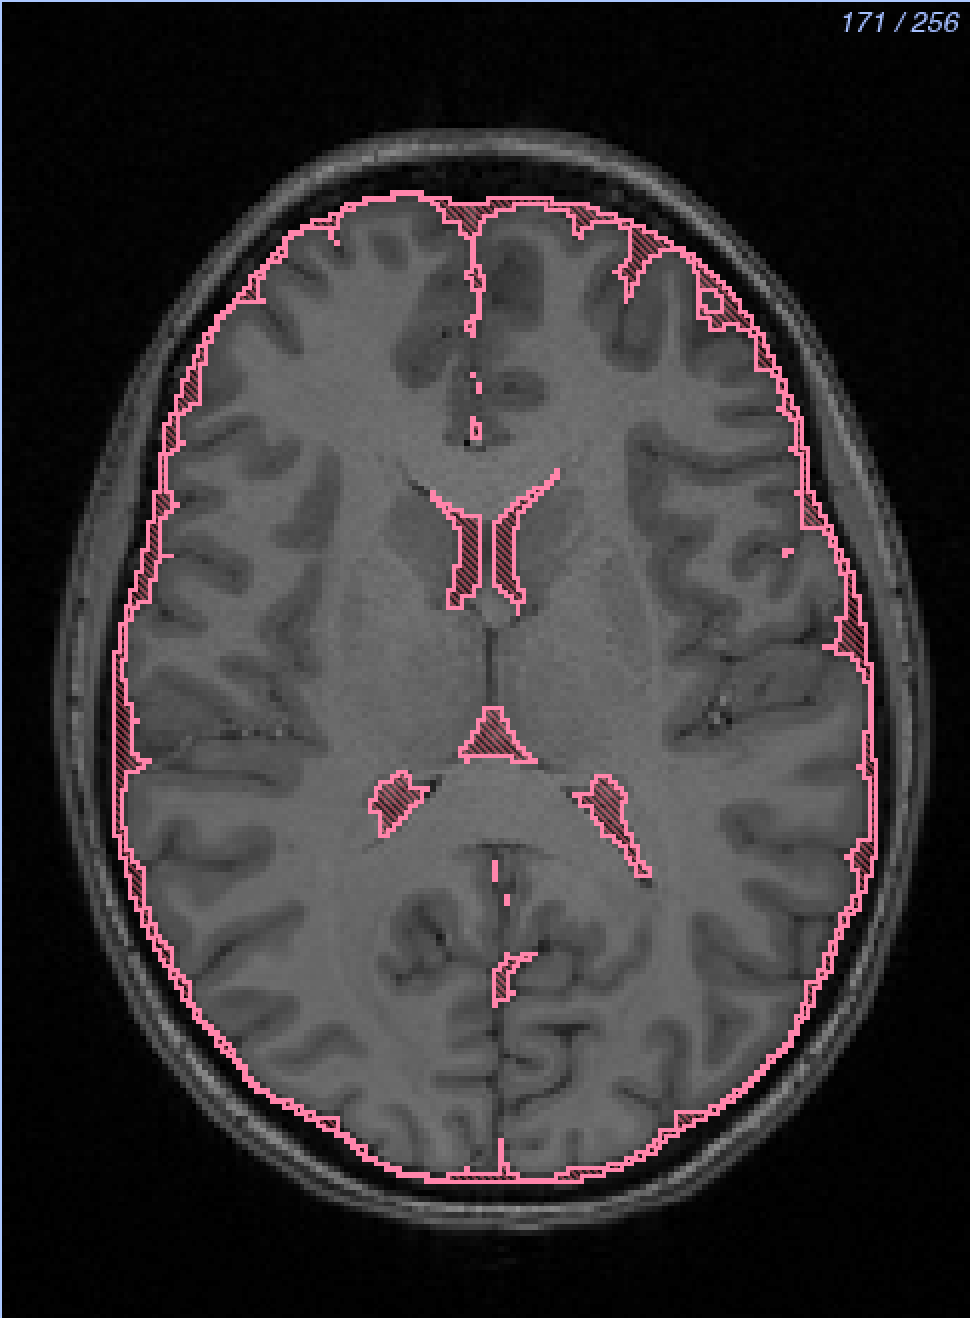
\includegraphics[width=.49\textwidth]{Figures/CSF_seg}
\caption{CSF segmentation.}
\label{fig:csf}
\end{center}
\end{figure}

The skull and the sinus layers were the most difficult to segment using only an MRI, because they both appear black in the MR image, and the subject's data did not include a computed tomography (CT) scan. For our first attempt to create a bone layer, we used FSL's BET2 tool (Figure \ref{fig:bet2}) to extract a skull surface. We then thresholded the $T_1$ MRI to create the remainder of the bones in Seg3D and connected the bones to the skull made from FSL. Although this approach gave an adequate segmentation for the skull, it did not include some important features, such as the sinus layer. As a second method, we estimated the skull from an MR-based synthetic pseudo-CT (Figure \ref{fig:ct}). We used an improved iterative version of the patch-based method as described by Torrado-Carvajal et al. \cite{ref:pseudoct} that takes the $T_1$ and $T_2$ images as input and synthesizes the pseudo-CT based on both images, providing more refined and accurate bone boundaries.

\begin{figure}[H]
\begin{center}
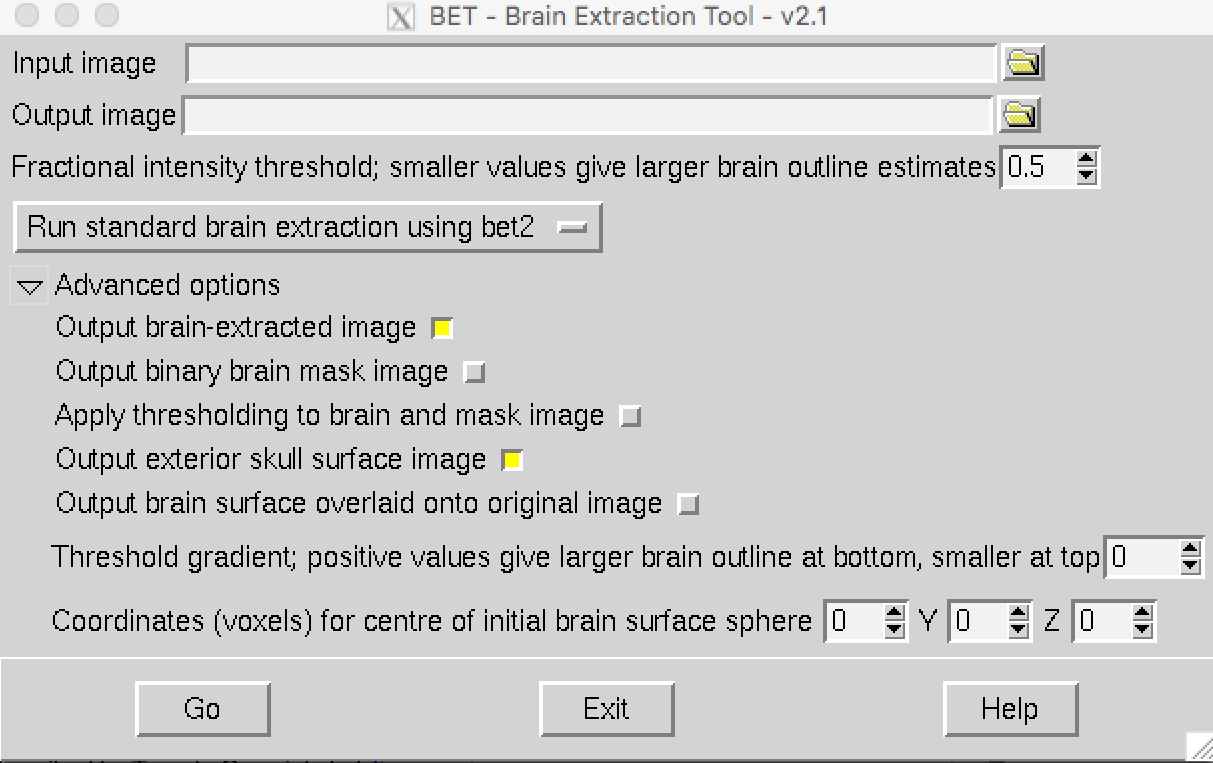
\includegraphics[width=.75\textwidth]{Figures/BET2}
\caption{FSL's BET2 tool.}
\label{fig:bet2}
\end{center}
\end{figure}

\begin{figure}[H]
\begin{center}
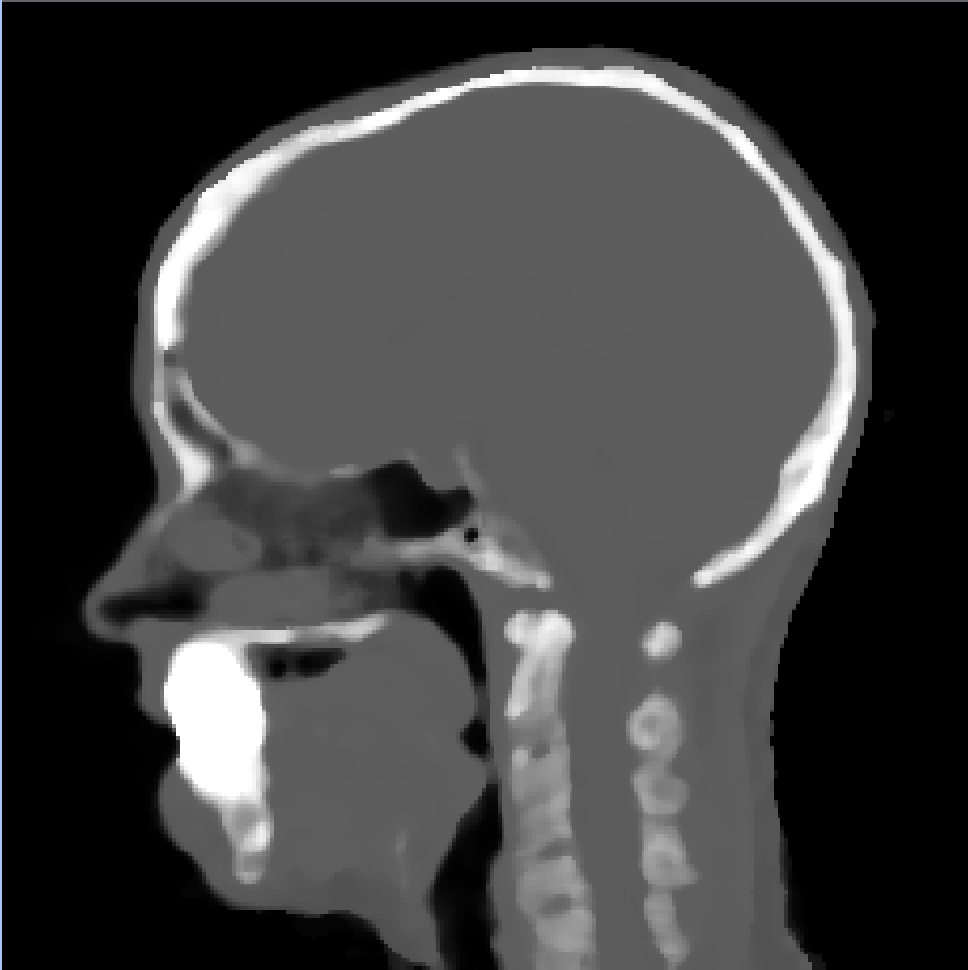
\includegraphics[width=.64\textwidth]{Figures/pseudo_CT}
\caption{Pseudo-CT scan.}
\label{fig:ct}
\end{center}
\end{figure}

The pseudo-CT method provided an image that was an easier starting place for skull segmentation, but we still manually edited the layer to add detail. After we applied a median filter with a one-pixel radius and thresholded the skull segmentation, we manually edited each slice in every direction to add detail and to smooth noisy sections of the layer. Since the subject had a permanent retainer in her mouth that created all black pixels, we segmented the mouth as solid bone, which we deemed acceptable because the EEG cap used did not cover the subject's mouth. We were able to provide a segmentation of the internal air, including the sinuses, esophagus, and ear canals, from the pseudo-CT image by thresholding the black pixels and then manually editing each slice. We also performed a quality check on both layers to ensure they had no holes or layer overlap and that they were at least two pixels thick.

The eyes, skin, and air layers were the least time consuming to segment. We segmented the eyes by thresholding the $T_2$ MRI. We segmented the skin layer by thresholding the entire head volume and removing all previous layers using a Boolean remove mask filter. We performed a quality check on the skin layer to ensure that it was at least two pixels thick. The areas that required significant correction were the bridge of the nose, the bottom of the chin, and the sides of the head. Lastly, we included pixels not previously assigned as the air layer. We checked through the entire segmentation to ensure that there weren't any holes between layers to assure a quality mesh and accurate simulation results. 

The complete head model presented here took approximately one year to complete, in part due to the many options in software and techniques, as well as the complexity of the multimodal imaging data. The segmentation of the image data took approximately 100 hours, mostly dedicated to manual editing.

\begin{table}[H]
\centering
\caption{Segmentation Time}
\label{tab:seg}
\begin{tabular}{|c|c|}
\hline
Segmented Tissue    & Amount of Work (hrs) \\ \hline
White Matter       & 40                   \\ \hline
Gray Matter         & 20                   \\ \hline
CSF                 & 4                    \\ \hline
Skull and Sinus     & 35                   \\ \hline
Eyes, Scalp, \& Air & 8                    \\ \hline
\end{tabular}
\end{table}

\subsection{Mesh Generation}
\label{sec:mesh}

%%% Settings for mesh generation, issues 

We used our full-head segmentation to generate realistic three-dimensional geometries for use in subsequent finite element simulations. We generated a smooth, linear, subject-specific, boundary-conforming, tetrahedral mesh using the Cleaver software \cite{ref:cleaver} on a Late 2013 Mac Pro with a 2.7 Ghz 12 Core Intel Xeon E5 processor with 64 GB of RAM and an AMD FirePro graphics card. Cleaver is a multimaterial meshing package that produces structured meshes of tetrahedral elements with guaranteed minimum element angles, resulting in quality meshes that require fewer computational resources. We made a high-resolution mesh without holes using the parameters listed in Table \ref{tab:cleaver}.
\begin{table}[H]
\centering
\caption{Clever Settings (High Resolution)}
\label{tab:cleaver}
\begin{tabular}{|c|c|}
\hline
scaling factor                    & 0.6                 \\ \hline
size multiplier                   & 1.0                 \\ \hline
lipschitz                         & 0.2                 \\ \hline
padding                           & 0                   \\ \hline
element sizing method             & adaptive            \\ \hline
\end{tabular}
\end{table}

We created indicator functions, functions describing the location of the surface with sub grid accuracy, by calculating inverted distance maps of each layer in the full-head segmentation in Seg3D. To reduce the size of the mesh, we first generated a new mesh, changing only the scaling factor parameter to 1.0 from the parameters in Table \ref{tab:cleaver}. We exported the computing sizing field from Cleaver and manipulated it in SCIRun by changing how quickly the elements increased in size. We input the changed sizing field into Cleaver with the same indicator functions and successfully cleaved a new, smaller mesh without holes.

\subsection{Mathematical Modeling}
\label{sec:math}

%%%MATH

The forward and inverse EEG problems are governed by a generalized Poisson equation (\ref{eq:1}). We used the head mesh, with associated inhomogeneous and anisotropic conductivity regions, as a volume conductor to solve the following boundary value problem:
%
\begin{equation}
\label{eq:1} \nabla\cdot\sigma\nabla\Phi = -I_{V} \;\;\;\;\mbox{ in
}\Omega,
\end{equation} 
%
where $\Phi$ is the electrostatic potential, $\sigma$ is the electrical conductivity tensor, and $I_{V}$ is the current per unit volume defined within the solution domain, $\Omega$. For the forward EEG problem, equation \ref{eq:1} was solved for $\Phi$ with a known description of $I_{V}$ and the Neumann boundary condition:
%
\begin{equation} \sigma\nabla\Phi\cdot{\bf
n} = 0\;\;\;\;\;\mbox{ on }\Gamma_{H}, 
\end{equation} 
%
which says that the normal component of the electric field is zero on the surface interfacing with air (here denoted by $\Gamma_{H}$). For testing purposes, we used dipoles for the current source. We calculated the electrical and potential fields everywhere within the head model. \cite{SCI:Joh2015c}

\subsubsection{Electrical Conductivity Preparation}
\label{sec:cond}

All electrical conductivities were homogeneous for each tissue with the exception of the white matter when using DTI data. The isotropic conductivities \cite{ref:cond} we used are shown in Table \ref{tab:cond}.

\begin{table}[H]
\centering
\caption{Isotropic Tissue Conductivity}
\label{tab:cond}
\begin{tabular}{|c|c|}
\hline
Tissue Type               & Isotropic Conductivity $(S/m)$ \\ \hline
\hline
White Matter              & 0.1429                         \\ \hline
Gray Matter               & 0.3333                         \\ \hline
Cerebrospinal Fluid (CSF) & 1.79                           \\ \hline
Skull                     & 0.001                          \\ \hline
Skin                      & 0.4346                         \\ \hline
Sinus                     & 1e-6                           \\ \hline
Eyes                      & 0.5051                         \\ \hline
\end{tabular}
\end{table}

When we added the DTI tensor data, we used two approaches to convert the tensor data to conductivities. The first was scaling the data \cite{ref:scaling}: 

\begin{equation}
\label{eq:scaling}
\sigma_{aniso} = \frac{\sigma_{iso}}{\sqrt[3]{d_1d_2d_3}}D,
\end{equation}
where $D$ is the diffusion data, $d_i$ is the $i$th eigenvalue of $D$, and $\sigma_{iso}$ is the white matter isotropic conductivity. The second method gave the white matter a fixed ratio of conductivity:

\begin{equation}
\label{eq:fixed}
\sigma_{aniso} = \begin{bmatrix}
v_1\\
v_2\\
v_3\\
W\\
\end{bmatrix}, 
W = \begin{bmatrix}
\sigma_{iso}\\
\frac{\sigma_{iso}}{10}\\
\frac{\sigma_{iso}}{10}\\
\end{bmatrix},
\end{equation}
where $v_i$ is the $i$th eigenvector of $D$, $W$ is the white matter ratio vector, and the ratio is $10:1$.

We implemented both methods into the SCIRun networks for anisotropic forward problems (\ref{fig:anisofornet}). 

\subsubsection{Numerical Methods}
\label{sec:numerical}

%%% This paragraph addresses Finite Element Discretization

We computed solutions to equation \ref{eq:1} using the finite element method. By applying Green's theorem to equation \ref{eq:1}, we generated the following weak formulation,
\begin{equation}
\label{eq:weakGreens}
\langle \sigma \nabla \phi, \nabla \bar{\phi} \rangle = -\langle I_v, \bar{\phi} \rangle
\end{equation}
where $ \bar{\phi}$ is an arbitrary test function, which can be thought of physically as a virtual potential field. By applying the Galerkin approximation to equation \ref{eq:weakGreens}, we can represent the finite element approximation as:
\begin{equation}
\label{eq:galerkin}
\sum_{i = 0}^{N} \varepsilon_i \langle \sigma_{ij} \nabla \psi_{i}, \nabla \psi_{j} \rangle = -\langle I_v, \psi_i \rangle \quad j = 0, \dots, N,
\end{equation}
subject to the Dirichlet boundary condition. Then the finite element approximation of equation \ref{eq:1} can equivalently be expressed as a system of $N$ equations with $N$ unknowns $\varepsilon_i \dots \varepsilon_N$ (e.g., the electrostatic potentials). In matrix form, the above system can be written as $A \varepsilon = b$,  where $A=(a_{ij})$ is called the global stiffness matrix and has elements $(a_{ij}) = (\sigma_{ij} \nabla \psi_{i}, \nabla \psi_{j})$, and $b_i = -(I_v, \psi_i)$ is usually termed the load vector. For volume conductor problems, $A$ contains all the geometry and conductivity information of the model. \cite{SCI:Joh2015c}

%%% This paragraph addresses SCIRun as a solver
We used SCIRun, the open-source problem-solving environment, to apply parameters and to solve equation \ref{eq:galerkin} numerically using linear basis functions for tetrahedral elements. Within the SCIRun environment, we applied isotropic and anisotropic conductivity tensors to the tetrahedral mesh as well as to inhomogeneous regions. We applied Dirichlet and Neumann boundary conditions to compute potentials using a conjugate gradient method with a Jacobi preconditioner.

\subsection{Simulations and Visualizations}
\label{sec:sim}

We ran all simulations and visualizations in the SCIRun problem-solving environment. All networks are shown in the Appendix in Section \ref{sec:networks} - Figures \ref{fig:maketensornet} - \ref{fig:eegvisnet}.

\subsubsection{Forward Problem}

Solving systems from a known source to the EEG electrodes, described in Section 2.5, is known as a forward problem. The opposite action, solving systems from the EEG data to a unknown source, is an inverse problem.  In this project, we built SCIRun example networks to solve forward problems with known sources and to write a lead field matrix for use in future inverse problems. We solved forward problems with an isotropic and anisotropic conductivities, using iDTI data for the direction for anisotropic conductivities.

The required inputs for the isotropic example network were the tetrahedral head mesh, isotropic conductivities, the head segmentation, the physical electrode locations, and dipole sources. The physical electrode locations and the dipole sources were results from the EEG recording dataset, and contained 4800 dipoles and the choice of 128 electrodes or 256 electrodes. The SCIRun network allowed the user to choose a dipole as a current source from the dataset for a forward simulation. The network also removed fiducial electrodes from the dataset. We registered the mesh to the head segmentation using a rigid registration previously described in Section \ref{sec:reg}. After we cut the flat tetrahedra out of the mesh, we mapped the conductivities to their respective tissues. We registered the electrodes and dipoles to the head mesh using the same transform. We solved the system with the mapped data and the chosen dipole sources. We then extracted the solution onto the head surface and the electrode locations for visualization. We also included streamlines and isopotential lines in the visualization.

For the anisotropic case, the network was largely the same with the exception of the scaled diffusion tensor dataset used as white matter conductivities. In addition, the DTI to mesh transform was needed as input. We registered the head mesh, electrodes, and dipoles to the DTI space with a rigid registration; the head segmentation was not needed.

\subsubsection{fMRI}

We visualized the fMRI data one time step at a time using the two-dimensional matrix described in Section \ref{sec:fmripre} as input by extracting one column at a time. We set each column onto a lattice volume, rotated it 180 degrees, smoothed, thresholded, and clipped the volume for easier rigid registration. We registered the fMRI to the tetrahedral mesh using the bounding boxes and manual registration. After registration, we mapped the smoothed fMRI data onto the mesh using a mapping matrix with a linear interpolation basis.

\subsubsection{EEG}

We visualized EEG data on the physical electrode locations, which we registered to the mesh space with a rigid registration after removing the fiducials from the electrode dataset. We displayed the filtered EEG signals one time step at a time by extracting the column of the matrix. We then placed the electrodes onto the mesh and mapped the EEG data onto the electrodes one time step at a time. The same network was used for both EEG data visualizations.

